% Inbuilt themes in beamer
\documentclass{beamer}

% Theme choice:
\usetheme{Berlin}
\usecolortheme{seahorse}

% packages
%\usepackage[hmargin=2cm, vmargin=2cm]{geometry}
\usepackage{microtype}
\usepackage{graphicx}
\usepackage{hyperref}
\usepackage[english]{babel}
\usepackage{setspace}
%\usepackage{xcolor}
\usepackage{multicol}
\usepackage{float}
\usepackage{amsmath}
\usepackage{amssymb}
\usepackage[font=small,skip=2pt]{caption}
\usepackage[
backend=biber,
style=authoryear-comp,
]{biblatex}

\addbibresource{../RMbibliography.bib}
\parindent=0pt

 \newcommand{\independent}{\perp\!\!\!\!\perp} 

% Title page details: 
\title{Scalar on Function Regression}
\author{Jonathan Willnow, Jakob Juergens, Jonghun Baek}
\date{{\color{red}}Presentation Day}

\begin{document}
	
	% Title page frame
	\begin{frame}
		\titlepage 
	\end{frame}
	
	% Remove logo from the next slides
	\logo{}
	
	% I'm not really a fan of a table of contents in short presentations (Jakob)
	% Outline frame
	%\begin{frame}{Outline}
	%	\tableofcontents
	%\end{frame}
	
	\begin{frame}{Introduction}
	
		\begin{itemize}
			\item Near-infrared (NIR) spectroscopy enables fast diagnostics by using the NIR region of the electromagnetic spectrum
			\item Suited for field-monitoring / on-line analysis and diagnostics of e.g: prediction of octane ratings!
			\item Spectroscopy results in high-dimensional dataset.	
			\item This set of measurements along a continuum can be viewed as set of smooth spectral curves
			\item Regression to determine relationship between octane rating and spectral curves
			\end{itemize}
	\end{frame}
	
	\begin{frame}{Theory}
		A simple functional dataset is given by 
		$$\{x_{i}(t_{j,i}) \in \mathbb{R} \: \vert \: i = 1,2,...,N, \; j = 1,2,..., J_i, \; t_{j,i} \in [T_1, T_2] \}$$
		
		\begin{itemize}
			\item Continuous underlying process, where $x_i(t)$ exists $\forall t \in [T_1, T_2]$
			\item Only observed at $x_{i}(t_{j,i})$
			\item Growth curves, financial data, human perception (pitch), ...
			\item To abstract information from the curves, they must be interpretable!
			\end{itemize}
	\end{frame}

	\begin{frame}{Theory}
		Jonghun
		\begin{itemize}
			\item Random Functions (name square integrable functions)
			\item Motivate continuous stochastic processes (growth curves/electricity consumption/yield curves/stonks)
			\item Use curves to predict a scalar response (show typical dgp)
		\end{itemize}
	\end{frame}

	\begin{frame}{Theory}
		Jonghun
		\begin{itemize}
			\item Basis expansions (b-splines and fourier)
			\item Talk about purposes
			\item Plots and show bias variance tradeoff
		\end{itemize}
	\end{frame}

	\begin{frame}{Random Function}
		Random element is a function $X : \Omega \rightarrow \mathcal{S}$ which is defined on a common probability space $(\Omega, \mathcal{F}, \mathbb{P})$ where $\Omega$ is a probability space with a $\sigma$-algebra $\mathcal{F}$ and a probability measure $\mathbb{{P}}.$
		\begin{itemize}
			\item If $\mathcal{S} = \mathbb{R}$ $\rightarrow$ X is a random variable
			\item If $\mathcal{S} = \mathbb{R}^{n}$ $\rightarrow$ X is a random vector
			\item If $\mathcal{S}$ is a space of functions, $X$ is called a random function
		\end{itemize}
	\end{frame}

	\begin{frame}{Random Function}
		Let $E$ be the index set and this can be described as
		$${\{X(t,\omega) : t \in E, \omega \in \Omega\},}$$
		where $X(t, \cdot)$ is $\mathcal{F}$-measurable function on the sample space $\Omega$.\\
		\begin{itemize}
			\item It can be shortened to $X(t)$ by omitting $\omega$
			\item The function is realized when the $X(t)$ have been observed for every $t \in E$
		\end{itemize}
	\end{frame}
	
	\begin{frame}{Square Integrable Function}
		If a function $f$ satisfies:
		$$\int_{0}^{1} \{f(t)\}^{2}dt < \infty$$
		the function $f$ is called square integrable function
		\begin{itemize}
			\item Without loss of generality, the interval is defined in $[0,1] $
			\item $\mathbb{L}^{2}$ is the set of all square integrable functions
			\item We focus on $\mathbb{L}^{2} [0,1]$ since the domain of our function is on the real line.
		\end{itemize}
	\end{frame}
	
	\begin{frame}{Square Integrable Function}
		If $f, g \in \mathbb{L}^{2}$,
		$$(ab + bg)(t) = af(t) + bg(t), \quad t \in [0,1] and \forall a,b$$
		, where $a$ and $b$ are scalars. (Maybe don't need)\\
		We can additionally define the inner product as follows:
		$$\langle f,g \rangle = \int_{0}^{1} f(t)g(t)dt$$
		\begin{itemize}
			\item Orthogonolality of two different functions
			\item Distance between functions
		\end{itemize}
	\end{frame}
	
	\begin{frame}{Stochastic Process Perspective}
		Functional data are the sample curves observed from continuous time stochastic precess.\\
		\begin{itemize}
			\item From this perspective, $X(t)$ is a random variable (?)\\
			\item $X(\cdot)$ is a collection of random variables by each time index(?)\\
			\item Realizations of a random function belong in large collection of functions
		\end{itemize}		
	\end{frame}
	
	\begin{frame}{Plots}
		\begin{figure}
			\centering
			\begin{minipage}{.5\textwidth}
				\centering
				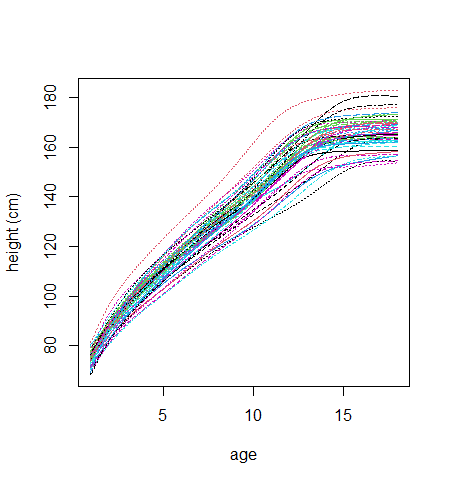
\includegraphics[width=\textwidth]{../Graphics/Growth_curves.png}
				\caption{\tiny Growth curves of 54 girls age 1-18}
			\end{minipage}%
			\begin{minipage}{.5\textwidth}
				\centering
				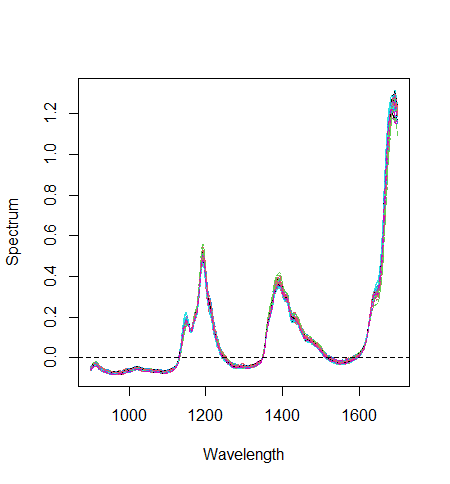
\includegraphics[width=\textwidth]{../Graphics/NIR.png}
				\caption {\tiny NIR spectrum of 60 gasoline samples}
			\end{minipage}
		\end{figure}
	\end{frame}
	
	\begin{frame}{Plots}
		point plots to link basis expansion
	\end{frame}
	\begin{frame}{Basis Expansion}
		Basis expansion is a linear combination of functions defining a function as described:
		$$X_{i}(t) \approx \sum_{k=1}^{K} c_{ik}\phi_{k}(t), \quad 1\leq i \leq n, \forall t \in E$$
		, where $\phi_{k}(t)$ is the $k^{th}$ basis function of the expansion and $c_{ik}$ is the corresponding coefficient.
		\begin{itemize}
			\item To make the function smoother
			\item To replace the original scalar data $X_{n}(t_{jn})$ by a smaller collection of $c_{nm}$
		\end{itemize}		
	\end{frame}
	
	\begin{frame}{Two Typical Types of Basis Function}
		Fourier basis function is written as
		$$f(x) = a_{0} + \sum_{n=1}^{\infty}a_{n}cos(2\pi nx) + b_{n}sin(2\pi nx)$$	\\
		\vspace{2\baselineskip}
		B-spline basis function is a flexible curve defined by degree and knots. \\
		Each B-spline basis function, $i$-th B-spline basis function of degree $p$, $N_{i,p}(u)$ is defined on Cox-de Boor recursion formula.(Do you think I need to put the formula?)
	\end{frame}
	
	\begin{frame}{Plots of Basis Functions}
		\begin{figure}
			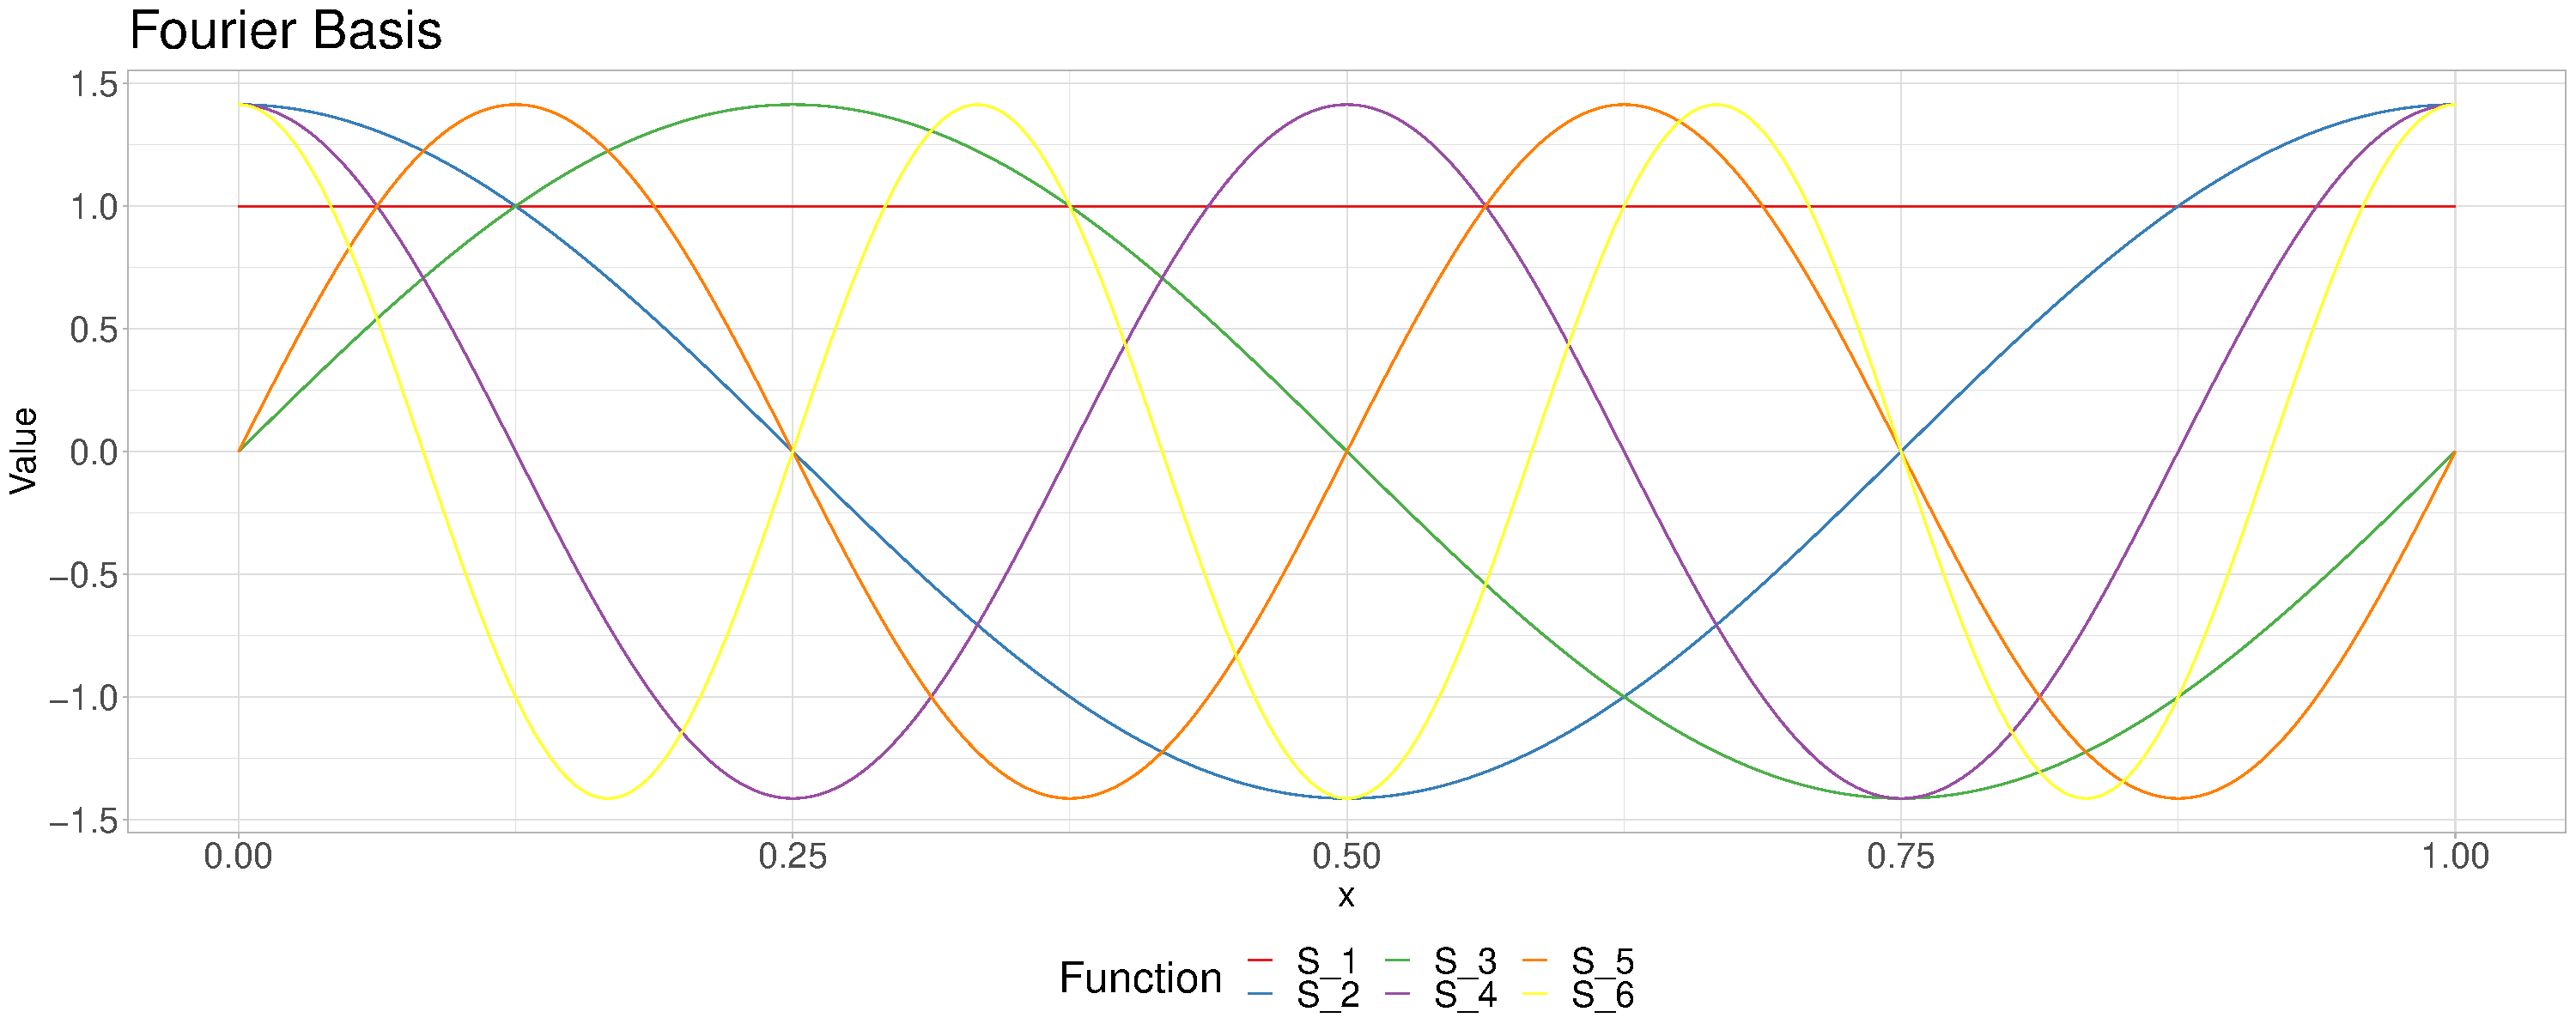
\includegraphics[height = 4.5cm]{../Graphics/Fourier_Basis.pdf}
			\caption {Fourier basis functions with order 9}
		\end{figure}
			
	\end{frame}
	
	\begin{frame}{Plots of Basis Functions}
		\begin{figure}
			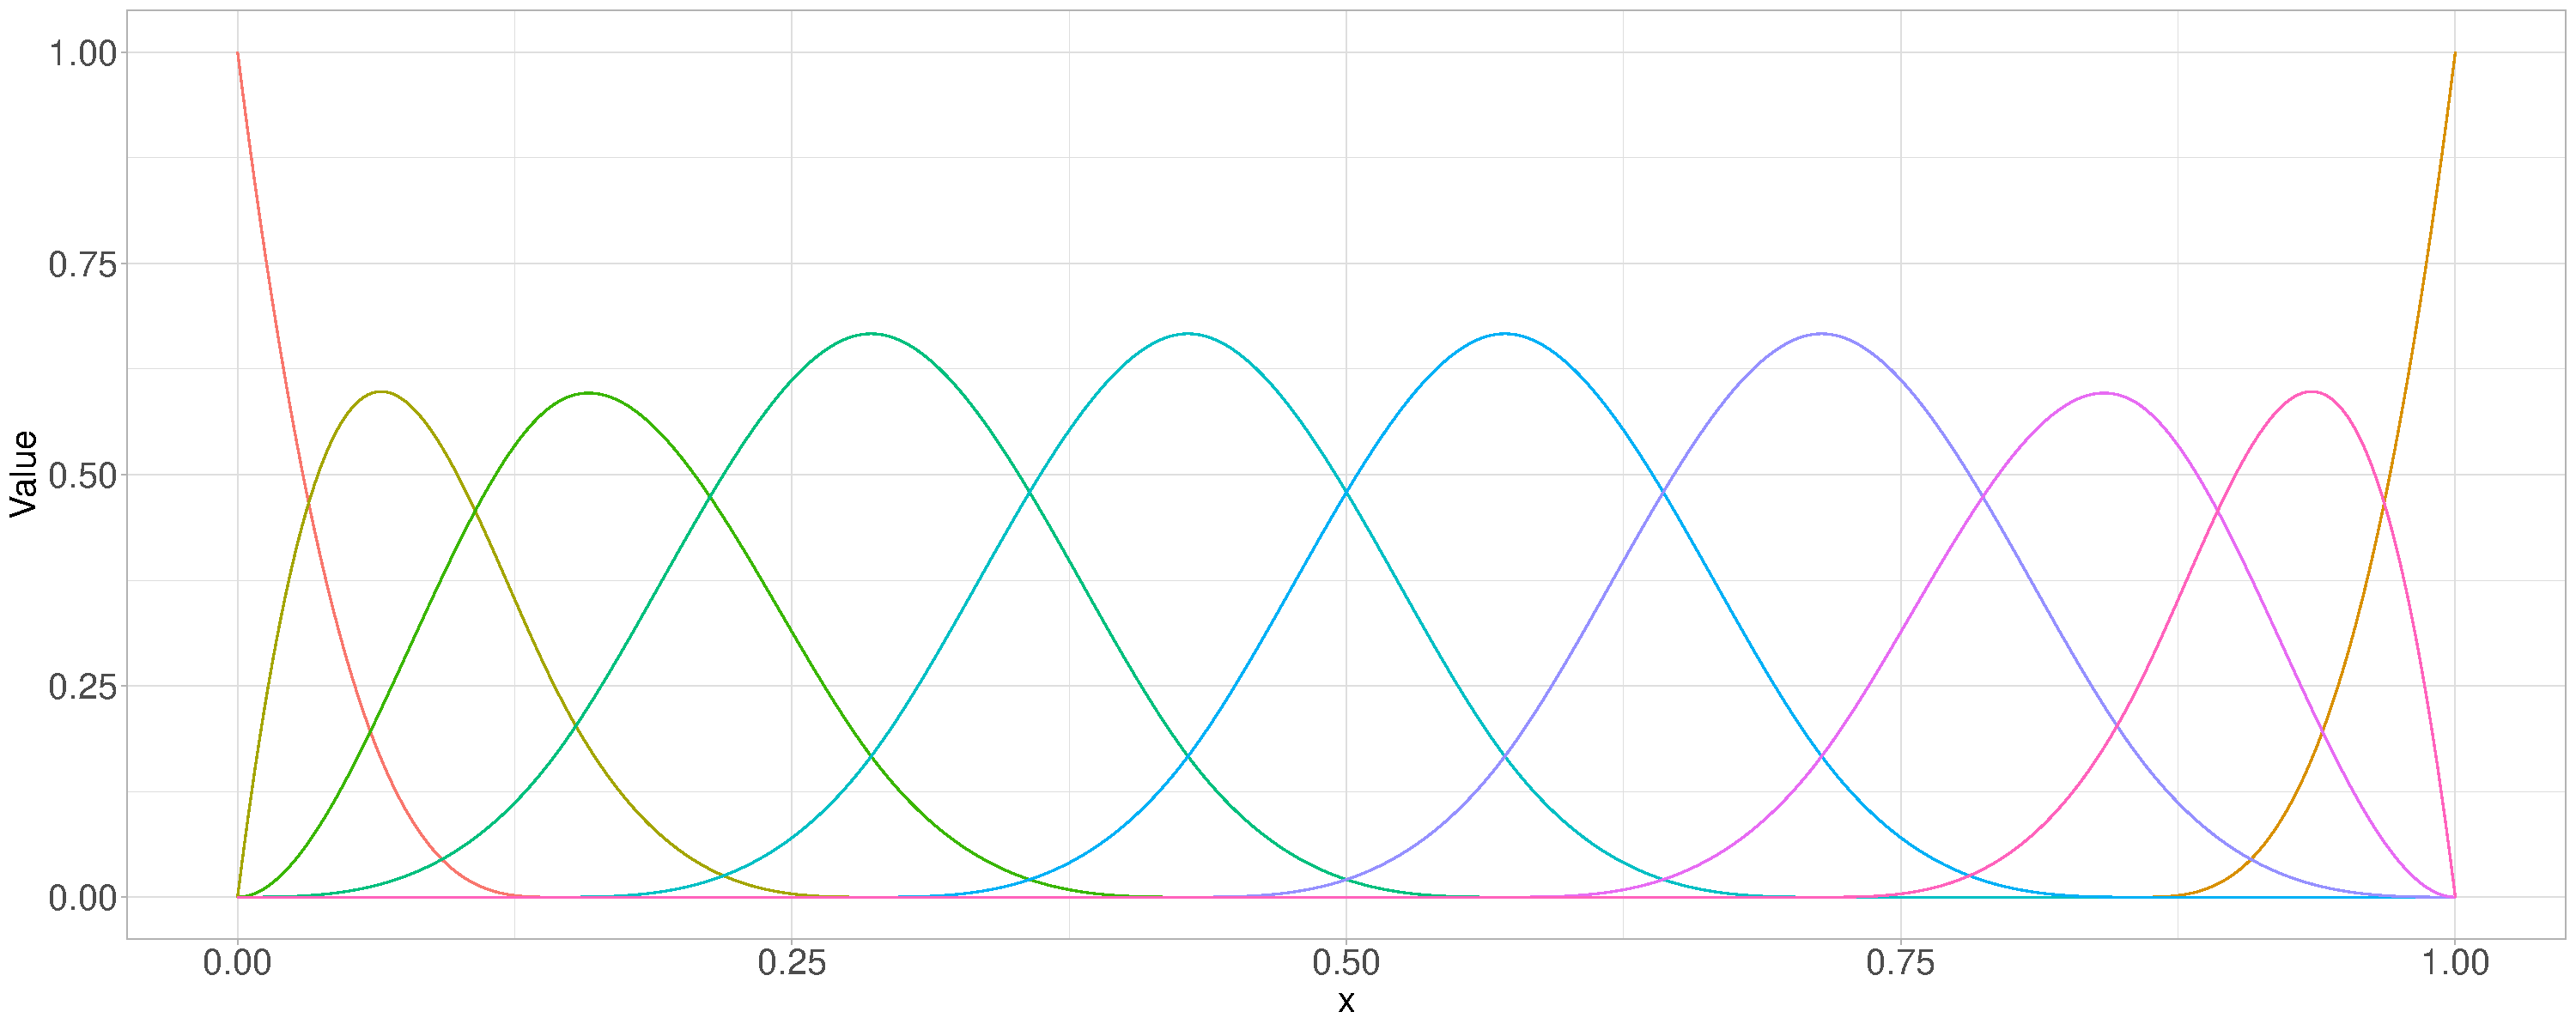
\includegraphics[height = 4.5cm]{../Graphics/Bspline_Basis.pdf}
			\caption {Bspline Basis with order 9}
		\end{figure}
	\end{frame}
	
	\begin{frame}{Trade Off between Bias and Variance}
		How do we choose the number $K$ of basis functions?
		\begin{itemize}
			\item The larger $K$, the better fit to the data with also fitting noise
			\item If $K$ is too small, it would miss some significant information that we want to estimate 
		\end{itemize}
	\end{frame}
	
	\begin{frame}{Trade Off between Bias and Variance}
		\begin{itemize}
			\item $\textbf{Bias}[\hat{x}(t)] = x(t) - E[\hat{x}(t)]$
			\item $\textbf{Var}[\hat{x}(t)] = E[\{\hat{x}(t) - E[x(t)]\}^2]$
			\item $\textbf{MSE}[\hat{x}(t)] = E[\{\hat{x}(t) - x(t)\}]$
			\item $\textbf{MSE}[\hat{x}(t)] = \textbf{Bias}^2[\hat{x}(t)] + \textbf{Var}[\hat{x}(t)]$
		\end{itemize}
		In the sense of that, we need to concentrate on decreasing \textbf{MSE}.
	\end{frame}
	
	\begin{frame}{Trade Off between Bias and Variance}
		\begin{minipage}[t]{\textwidth}
			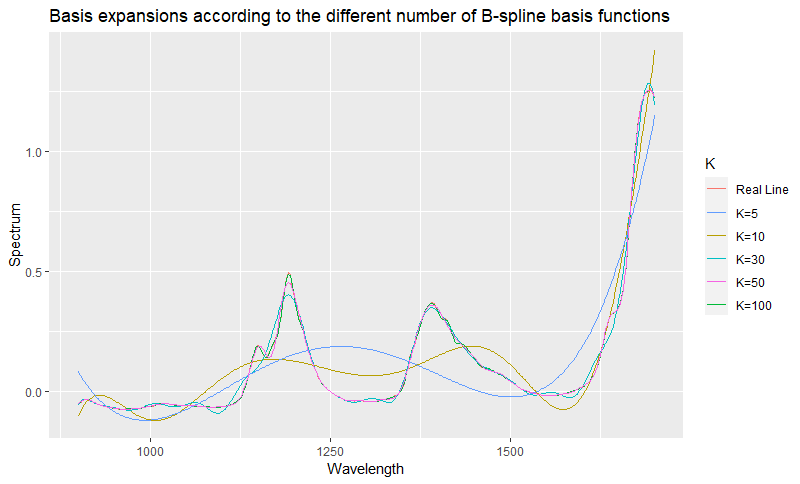
\includegraphics[height = 7cm]{../Graphics/Tradeoff.png}
		\end{minipage}
	\end{frame}

	%\begin{frame}{Theory}
	%	Jakob
	%	\begin{itemize}
	%		\item Random function represented as linear combination of basis functions $\checkmark$
	%		\item Just transform to multiple linear regression setting $\checkmark$
	%		\item You already know that from the beginning $\checkmark$
	%	\end{itemize}
	%\end{frame}

	\begin{frame}{Estimation via Basis Representation}
		Assume the following \textbf{data generating process}
		$$Y(\omega) = \alpha + \int_{0}^{1} \beta(s) F(\omega)(s) \mathrm{d}s + \epsilon(\omega)$$
		\begin{itemize}
			\item $Y(\omega)$ and $\epsilon(\omega)$ realize in $\mathbb{R}$ and $F(\omega)$ realizes in $\mathbb{L}^2[0,1]$
		\end{itemize}
		\vspace{0.2cm}
		
		Assume that we have a data set containing observations each of which is made up of:
		\begin{itemize}
			\item $y_i$: a scalar realization of $Y(\omega)$
			\item $f_i(t)$: a realization of $F(\omega)$
		\end{itemize}

	\end{frame}

	\begin{frame}{Estimation via Basis Representation}
		Let $\{b_i(t) \: \vert \: i = 1, \dots, \infty\}$ be a basis of $\mathbb{L}^2[0,1]$
		\vspace{0.2cm}
		
		Then we have the following representation of $\beta(t)$
		$$\beta(t) = \sum_{j = 1}^{\infty} \psi_j b_j(t) = \sum_{j = 1}^{L} \psi_j b_j(t) + \delta(t) \approx \sum_{j = 1}^{L} \psi_j b_j(t)$$
		and we can transform the data generating process into:
		\begin{equation}\notag
			\begin{split}
				Y(\omega) & = \alpha + \int_{0}^{1}\left[\left(\sum_{j = 1}^{\infty} \psi_j  b_j(s)\right) F(\omega)(s) \right]\mathrm{d}s + \epsilon(\omega) \\
						  & = \alpha + \sum_{j = 1}^{\infty} \left[\psi_j \textcolor{red}{\int_{0}^{1} F(\omega)(s) b_j(s)\mathrm{d}s}\right] + \epsilon(\omega)	  
			\end{split}
		\end{equation}
	\end{frame}

	\begin{frame}{Estimation via Basis Representation}
		$$Z_j(\omega) = \int_{0}^{1} F(\omega)(s) b_j(s)\mathrm{d}s$$ 
		This is a \textbf{scalar random variable} leading to the following transformation
		$$Y(\omega) = \alpha + \sum_{j = 1}^{\infty} \psi_j Z_j(\omega) + \epsilon(\omega)$$
		Each combination of observation $f_i(t)$ and deterministic basis function $b_j(t)$ effectively gives us a realization of this random variable.
		$$Z_{i,j} = \int_{0}^{1} f_i(s) b_j(s)\mathrm{d}s$$
		
	\end{frame}

	\begin{frame}{Estimation via Basis Representation}
		This allows us to write each observation in the data set as
		\begin{itemize}
			\item $y_i$: a scalar realization of $Y$
			\item $\left(Z_{i,j}\right)_{j \in \mathbb{N}}$: a countably infinite sequence of scalars
		\end{itemize}
		\vspace{0.2cm}
		
		Truncating the functional basis allows us to approximate the data set in the usual multivariate form.
		\begin{itemize}
			\item $y_i$: a scalar realization of $Y$
			\item $\left(Z_{i,1} \: \dots \:  Z_{i,L} \right)'$: a vector of scalar regressors
		\end{itemize}
		\vspace{0.2cm}
		
		Coefficients can then be estimated using theory from \textbf{multivariate regression} leading to an estimated coefficient vector $\hat{\psi}_L \in \mathbb{R}^L$.
	\end{frame}

	\begin{frame}{Estimation via Basis Representation}
		This can be translated into an estimated coefficient function $\hat{\beta}(t)$:
		
		$$\hat{\beta}_L(t) = \sum_{j = 1}^{L} \hat{\psi}_{L,j} b_j(t)$$
		\vspace{0.2cm}
	
		This is dependent on...
		\begin{itemize}
			\item The functional basis $(b_j(t))_{j \in \mathcal{I}}$ for the estimation of $\beta(t)$
			\item The truncation parameter $L$
			\item (The functional basis used to approximate the observations)
			\item (The truncation parameter in the approximation of the observations)
		\end{itemize}
	\end{frame}
	
	%\begin{frame}{Theory - FPCA}
	%	Jakob
	%	\begin{itemize}
	%		\item Let's assume you know the theory of PCA (pc from varcov matrix) $\checkmark$
	%		\item Introduce mean and covariance functions of random functions $\checkmark$
	%		\item There is another cool basis $\rightarrow$ Eigenbasis (Karhunen-Loeve Expansion) $\checkmark$
	%		\item Sample Analog! (create a basis from observations and use for basis regression) $\checkmark$
	%		\item Plot fpcs and approximation of function realization
	%	\end{itemize}
	%\end{frame}

	\begin{frame}{Spectral Representation of Random Vectors}
		Let $X(\omega)$ be a random vector realizing in $\mathbb{R}^p$.

		\begin{itemize}
			\item Let $\mu_x = \mathbb{E}(X)$ and $\Sigma_X = Cov(X)$
			\item Let $\{\gamma_i \: \vert \: i = 1, \dots, p\}$ be the orthonormal \textbf{Eigenvectors} of $\Sigma_X$
			\item Let $\{\lambda_i \: \vert \: i = 1, \dots, p\}$ be the corresponding \textbf{Eigenvalues} of $\Sigma_X$
		\end{itemize}
	
		\vspace{0.2cm}
		Then $X$ can also be represented as
		$$X(\omega) = \mu_x + \sum_{i = 1}^{p} \xi_i(\omega) \gamma_i$$
		where the $\xi_i(\omega)$ have the following properties
		
		\begin{multicols}{2}
			\begin{enumerate}
				\item $\mathbb{E}[\xi_i(\omega)] = 0$
				\item $Var(\xi_i(\omega)) = \lambda_i$
				\item $Cov(\xi_i(\omega), \xi_j(\omega)) = 0$ for $i \neq j$
			\end{enumerate}
		\end{multicols}
	\end{frame}

	\begin{frame}{Karhunen-Lo\'{e}ve Expansion}
		
		\textbf{Mean Function}: $$\mu(t) = \mathbb{E}\left[ F(\omega)(t) \right]$$

		\textbf{Autocovariance Function}: $$c(t,s) = \mathbb{E}\big[ \left( F(\omega)(t) - \mu(t) \right) \left( F(\omega)(s) - \mu(s) \right) \big]$$
		
		The \textbf{Eigenvalues} and \textbf{Eigenfunctions}: $\{(\lambda_i, \nu_i) \: \vert \: i \in \mathcal{I}\}$  are solutions of the following equation:
		$$ \int_{0}^{1}c(t,s)\nu(s) \mathrm{d}s = \lambda \nu(t) $$
	\end{frame}
	
	\begin{frame}{Karhunen-Lo\'{e}ve Expansion}
		A random function $F(\omega)$ can be expressed in terms of its mean function and its Eigenfunctions:
		$$F(\omega)(t) = \mu(t) + \sum_{j = 1}^{\infty} \xi_j(\omega) \nu_j(t)$$
		
		Where the $\xi_j$ are scalar-valued random variables with the following properties.
		\begin{multicols}{2}
			\begin{enumerate}
				\item $\mathbb{E}[\xi_i(\omega)] = 0$
				\item $Var(\xi_i(\omega)) = \lambda_i$
				\item $Cov(\xi_i(\omega), \xi_j(\omega)) = 0$ for $i \neq j$
			\end{enumerate}
		\end{multicols}
		
		This representation is called the \textbf{Karhunen-Lo\'{e}ve Expansion} of the random function $F$ and the Eigenfunctions can serve as a basis to represent the function.
	\end{frame}

	\begin{frame}{Principal Component Analysis}
		A related concept is \textbf{Principal Component Analysis} (PCA).
		\vspace{0.2cm}
		
		$\Sigma_X$ unknown $\rightarrow$ \textbf{sample analogues}
	
		\begin{itemize}
			\item Let $\mathbf{X} \in \mathbb{R}^{n \times p}$ contain the standardized regressors
			\item Let $\hat{\Sigma}_X = \frac{\mathbf{X}'\mathbf{X}}{n}$
			\item Let $\{\hat{\gamma}_i \: \vert \: i = 1, \dots, p\}$ be the orthonormal \textbf{Eigenvectors} of $\hat{\Sigma}_X$
			\item Let $\{\hat{\lambda}_i \: \vert \: i = 1, \dots, p\}$ be the corresponding \textbf{Eigenvalues} of $\hat{\Sigma}_X$
		\end{itemize}
		\vspace{0.2cm} 
		
		Then $Z_i(\omega) = \hat{\gamma}_i' X(\omega)$ is called the i'th principal component and
		\begin{multicols}{2}
			\begin{enumerate}
				\item $\mathbb{E}[Z_i(\omega)] = 0$
				\item $Var(Z_i(\omega)) = \hat{\lambda}_i$
				\item $Cov(Z_i(\omega), Z_j(\omega)) = 0$ for $i \neq j$
			\end{enumerate}
		\end{multicols}
	\end{frame}

	\begin{frame}{Functional Principal Component Analysis}
		This idea can be extended to functional regressors in the form of \textbf{Functional Principal Component Analysis} (FPCA).
		\vspace{0.2cm}
		
		\textbf{Empirical Mean Function}:
		$$\hat{\mu}(t) = \frac{1}{n}\sum_{j = 1}^{n}f_j(t)$$

		\textbf{Empirical Autocovariance Function}:
		$$\hat{c}(t,s) = \frac{1}{n} \sum_{j = 1}^{n} \left(f_j(t) - \hat{\mu}(t)\right) \left(f_j(s) - \hat{\mu}(s)\right)$$

	\end{frame}

	\begin{frame}{Functional Principal Component Analysis}
	
		The \textbf{Eigenvalues} and \textbf{Eigenfunctions}: $\{(\hat{\lambda}_i, \hat{\nu}_i) \: \vert \: i \in \mathcal{I}\}$  are solutions of the following equation:
		$$ \int_{0}^{1}\hat{c}(t,s)\hat{\nu}(s) \mathrm{d}s = \hat{\lambda} \hat{\nu}(t) $$
		\vspace{0.2cm}
		
		The $\{\hat{\nu}_i(s) \: \vert \: i \in \mathcal{I}\}$ are called \textbf{Functional Principal Components} and can serve as a basis for representing the original curves. 
		\vspace{0.2cm}
		
		The corresponding scores $\hat{\xi}_i$ can be derived as
		$$\hat{\xi}_j(\omega) = \int_{0}^{1} (F(\omega)(s) - \hat{\mu}(s)) \hat{\nu}_j(s) \mathrm{d}s$$
		
	\end{frame}

	\begin{frame}{FPCA - Plots}
		\begin{minipage}[c]{0.78\textwidth}
			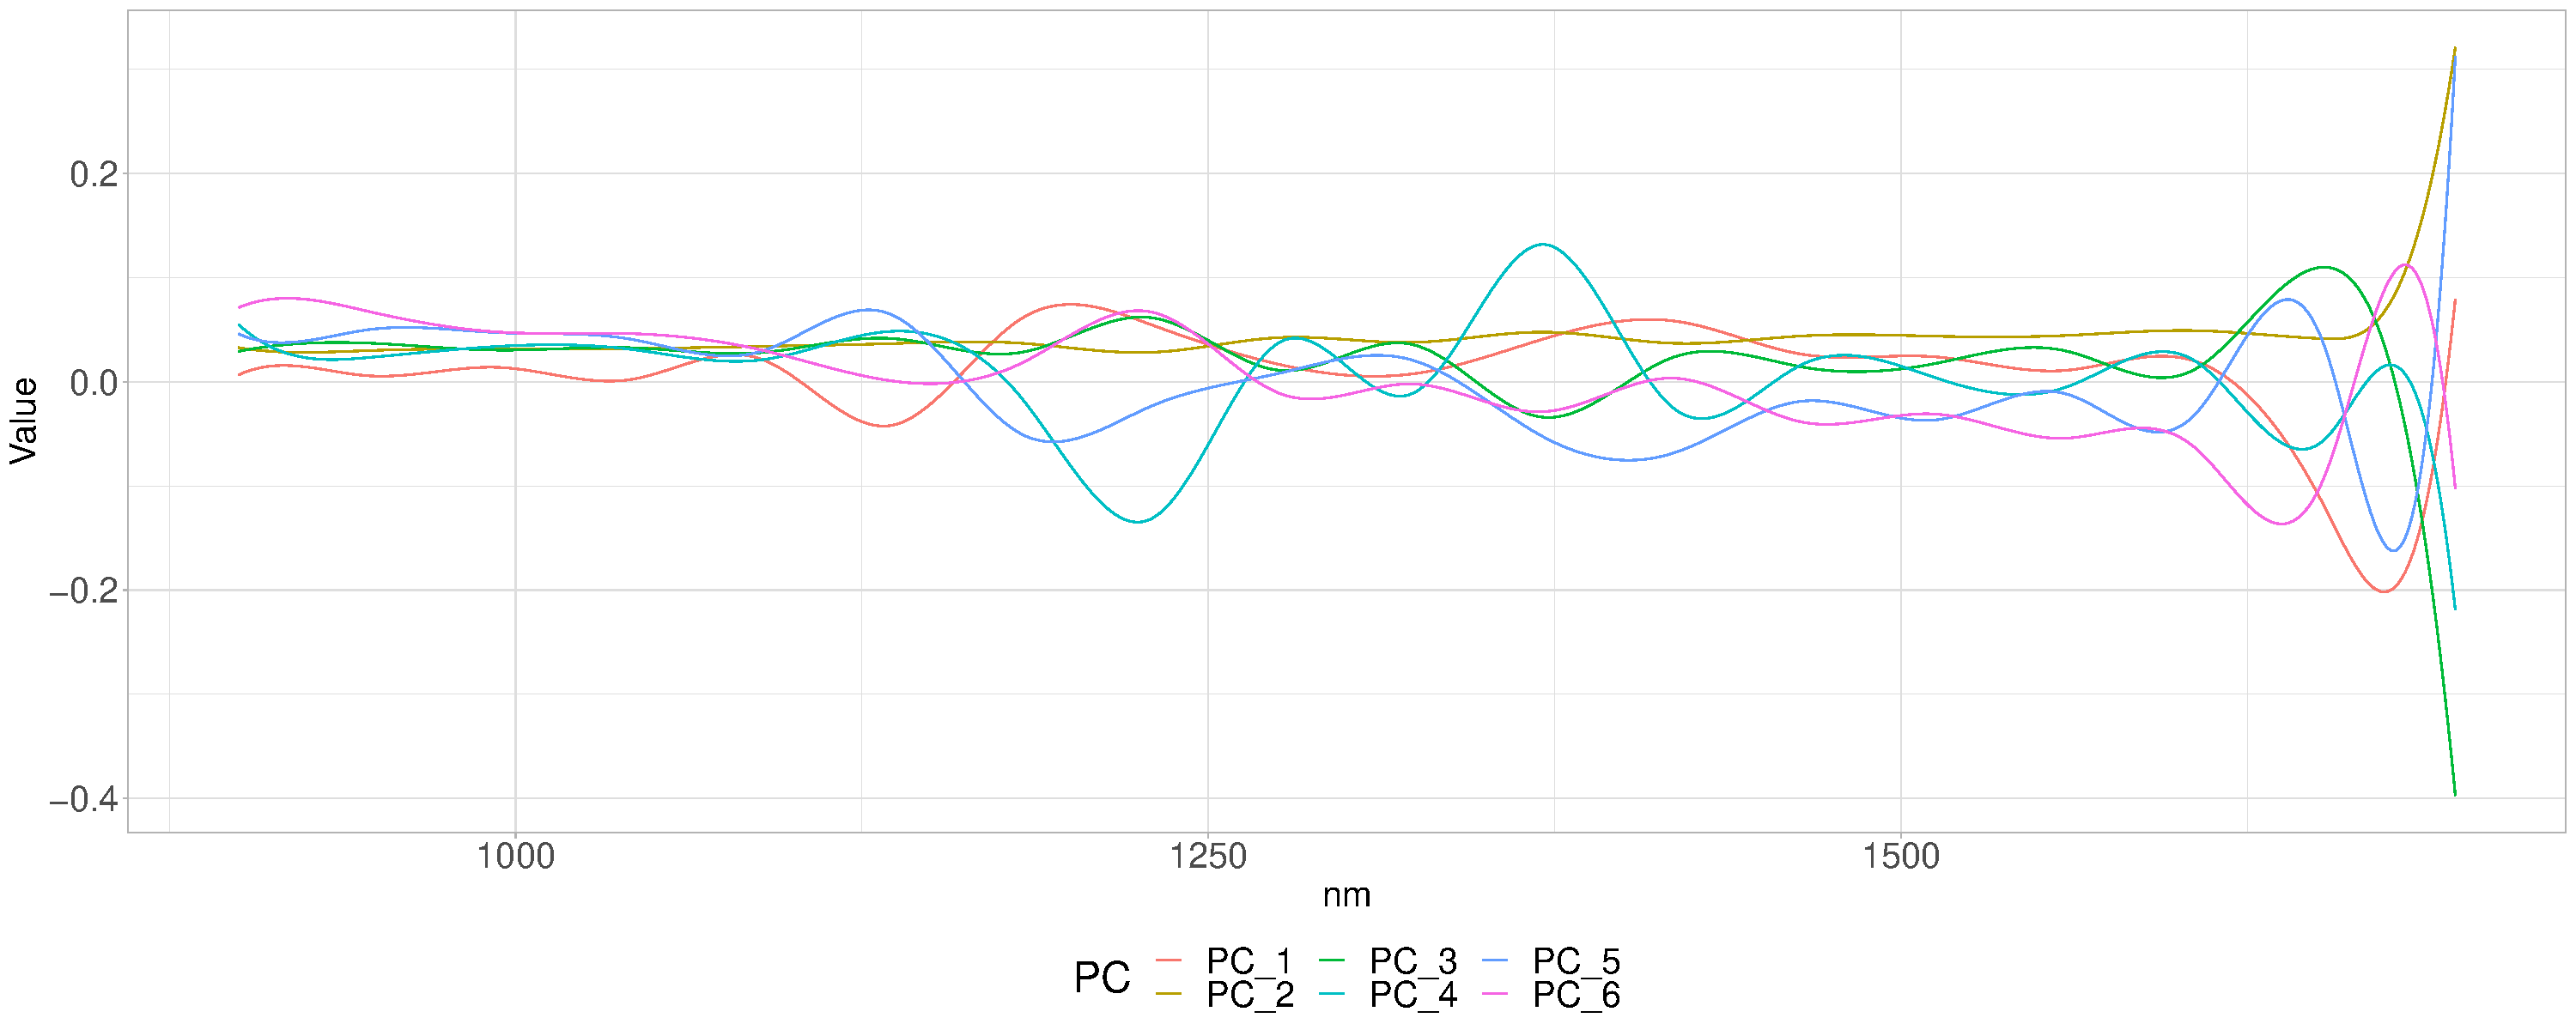
\includegraphics[width = \textwidth]{../Graphics/principal_components.pdf}
			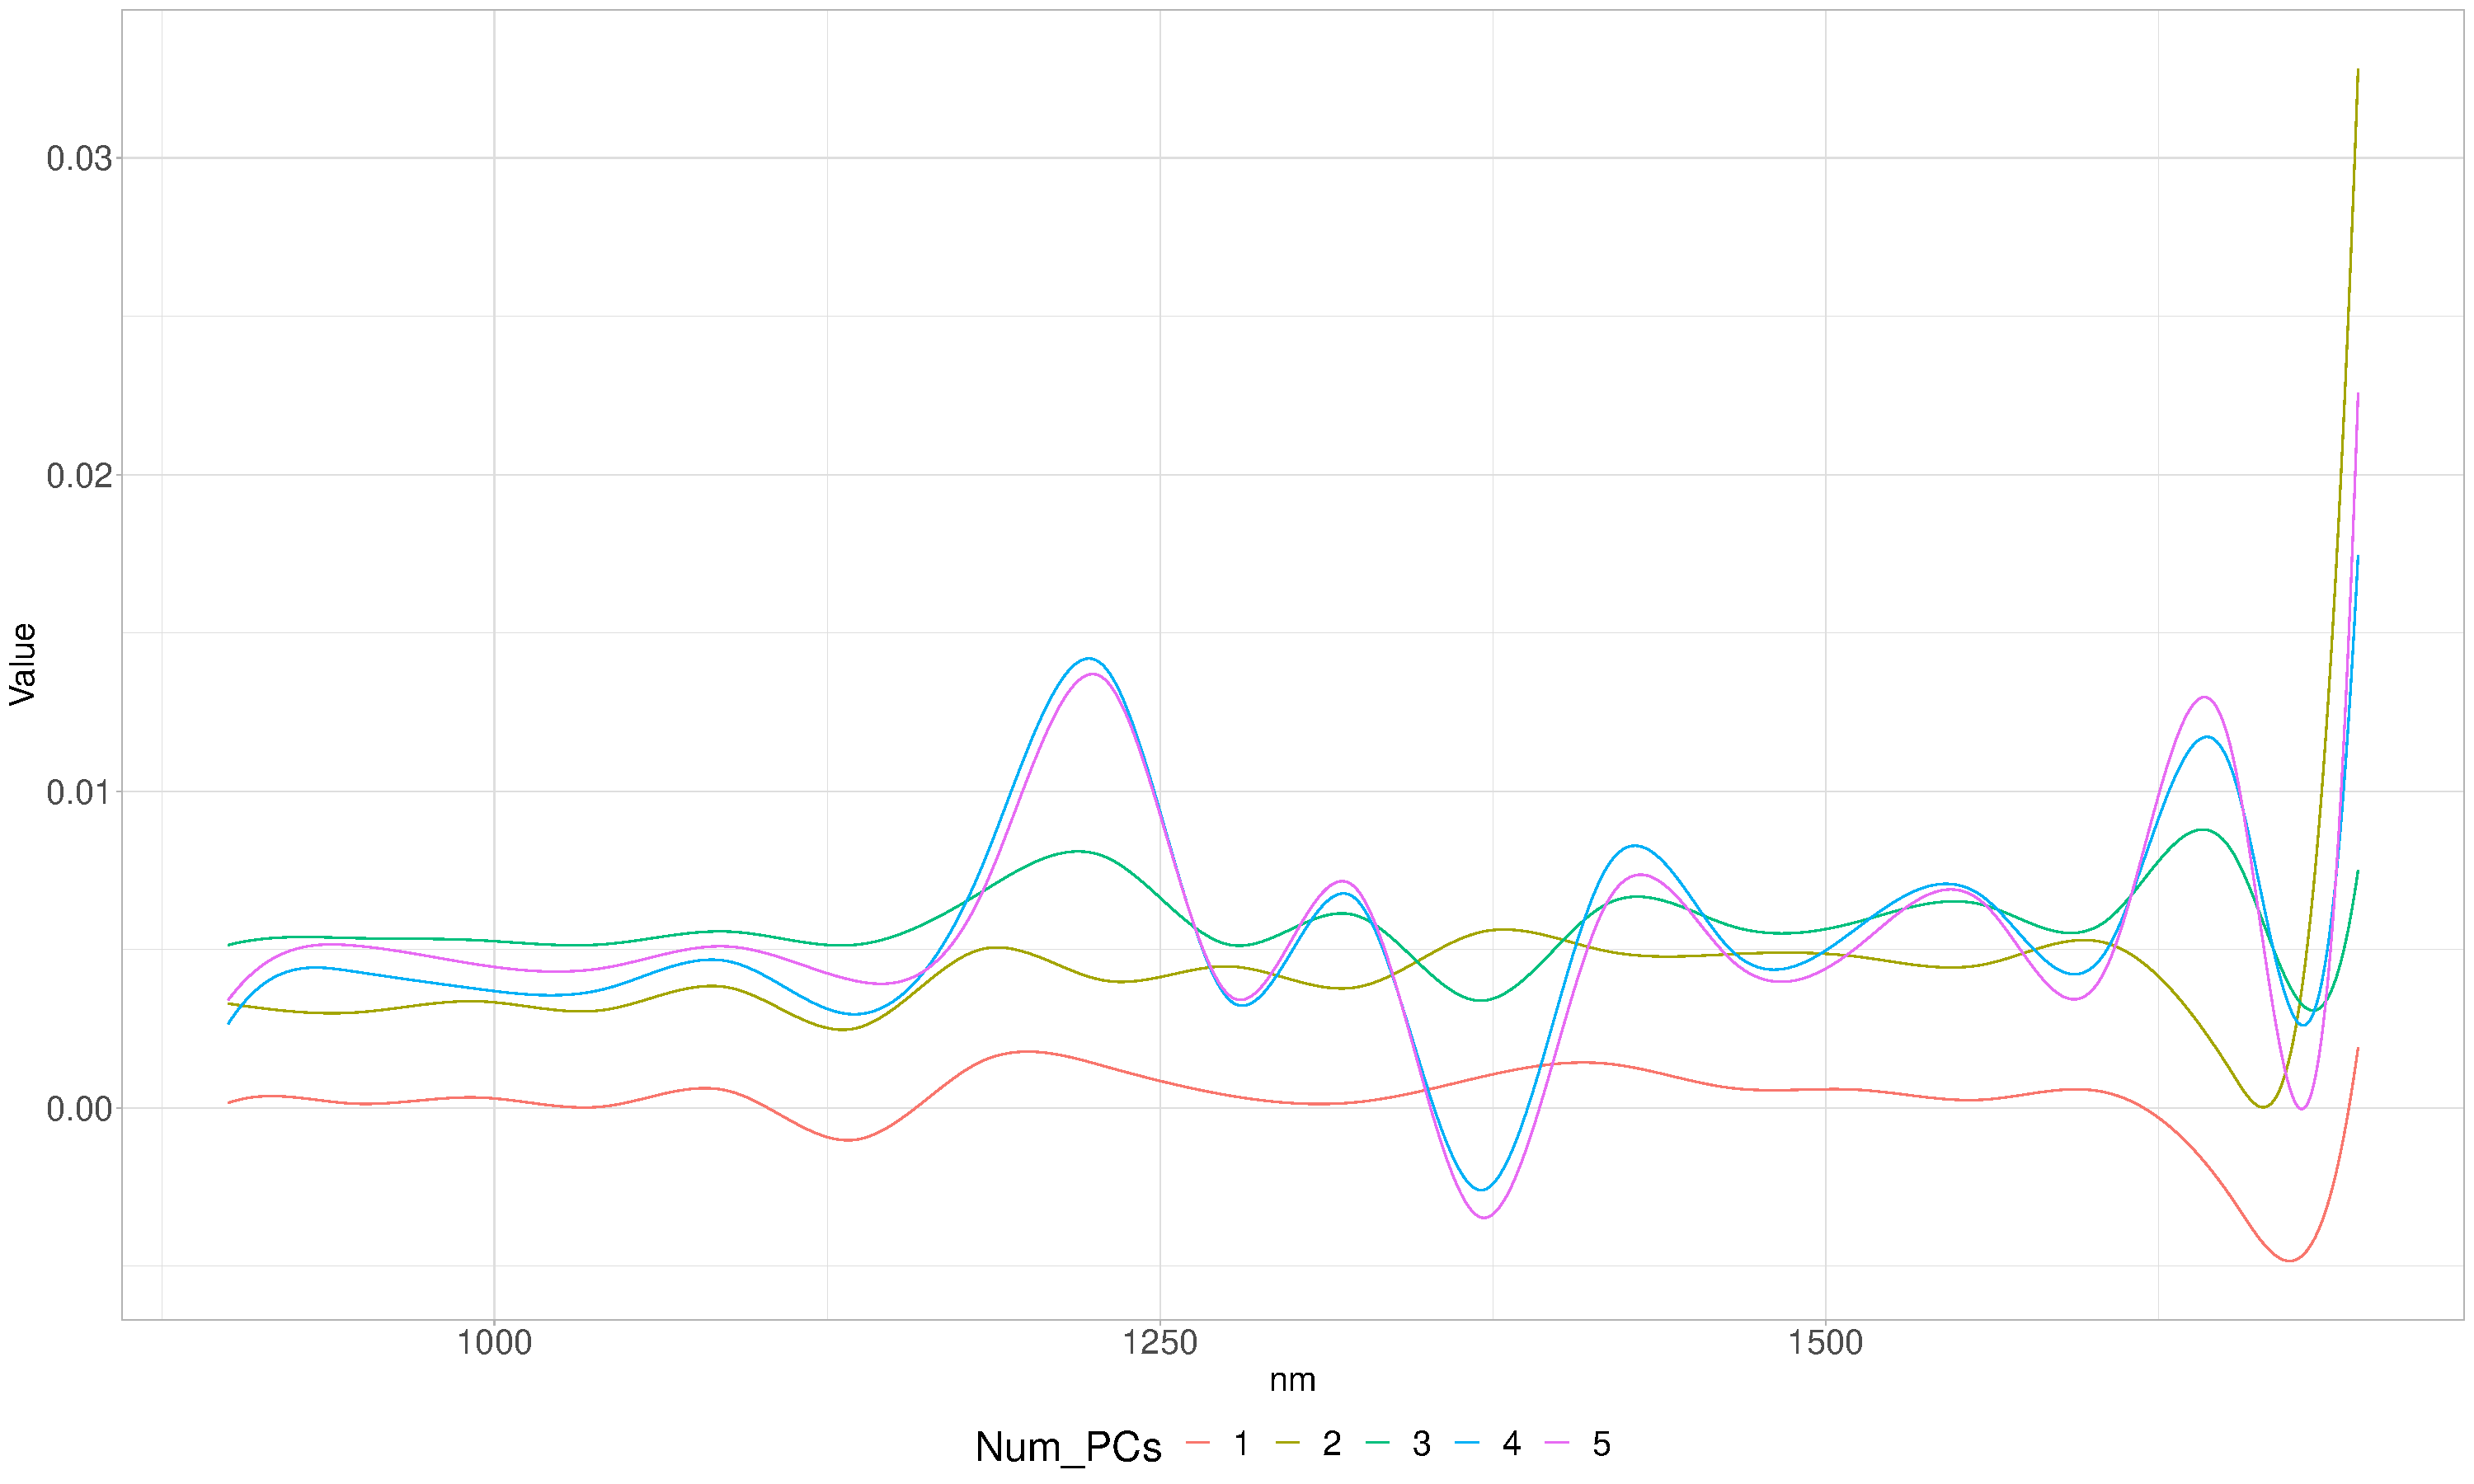
\includegraphics[width = \textwidth]{../Graphics/pc_approx.pdf}
		\end{minipage}
		\begin{minipage}[c]{0.19\textwidth}
			The math is for intuition. In practice there are problems and the fpc's are derived differently.
		\end{minipage}
	\end{frame}
	

	\begin{frame}{Simulation Setup \& Application}
		\begin{itemize}
			\item Use the \textbf{gasoline dataset} (NIR-spectroscopy, 60 $\times$ 401) to predict octane ratings.
			\item Generate \textbf{similar curves} from gasoline dataset:
		\end{itemize}
	
		$$\tilde{F}(\omega)(t) = \hat{\mu}(t) + \sum_{j = 1}^{\infty} \tilde{\xi}_j(\omega) \hat{\nu}_j(t)$$ 

		\begin{itemize}
			\item $\tilde{\xi}_{j} \sim \mathcal{N}(0,\hat{\lambda}_j)$ and $\tilde{\xi}_{j} \independent \tilde{\xi}_{k}$ for $j \neq k$
			\item Simplification: the $\xi_{j}$ do not follow a normal
			\item $\tilde{F}(\omega)(t)$, $\hat{\mu}(t)$ and $\hat{\nu}_j(t)$ are approximated as vectors in $\mathbb{R}^{401}$.
		\end{itemize}
		
	\end{frame}
	
	
	\begin{frame}{Simulation Setup \& Application cont.}
		%\begin{itemize}
		%\item
		Following \textbf{Reiss and Ogden (2007)}, let $f_1(t)$ and $f_2(t)$ be two coefficient functions: 
		%\vspace{0.2cm}

   		%$f_1(t) = 2\sin(0.5\pi t) + 4\sin(1.5 \pi t) + 5\sin(2.5 \pi t)$\\
   		%\vspace{0.1cm}
   		
        %$f_2(t) = 1.5 \exp(\frac{-0.5(t-0.3)^2}{0.02^2}) - 4 \exp(\frac{-0.5(t-0.45)^2}{0.015^2}) +  8 \exp(\frac{-0.5(t-0.6)^2}{0.02^2}) - \exp(\frac{-0.5(t-0.8)^2}{0.03^2})$
		
		%\end{itemize}
		\vspace{0.1cm}
		\begin{figure}
			\centering
			\begin{minipage}{.5\textwidth}
				\centering
  				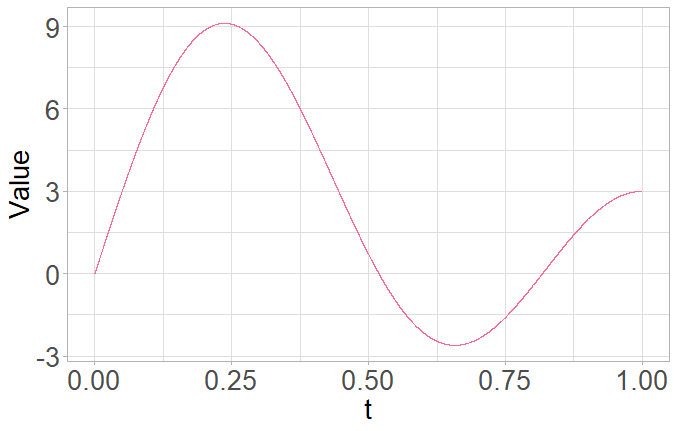
\includegraphics[width=\textwidth]{smooth_function.png}
  				\caption{$f_1(t)$, smooth function}
  				\label{fig:test1}
			\end{minipage}%
			\begin{minipage}{.5\textwidth}
	  			\centering
  				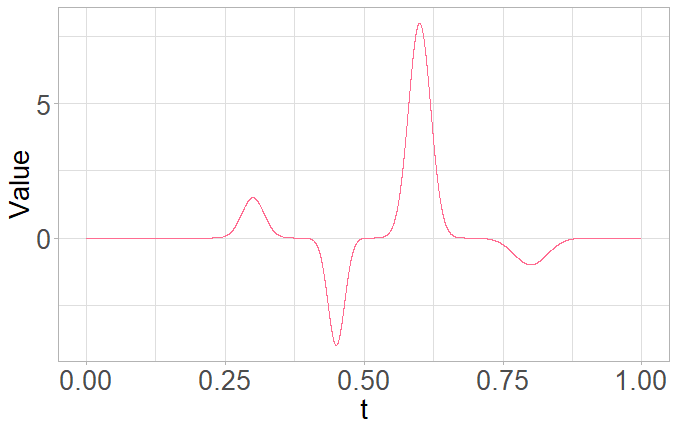
\includegraphics[width=\textwidth]{bumpy_function.png}
  				\caption{$f_2(t)$, bumpy function}
  				\label{fig:test2}
			\end{minipage}
		\end{figure}
		
	\end{frame}	

	
	\begin{frame}{Simulation Setup \& Application cont.}
		Let 
		$$Y_{1,f} = \langle NIR, f\rangle + Z  \frac{var(\langle NIR, f\rangle)}{0.9} - var(\langle NIR, f\rangle)$$ 
		$$Y_{2,f} = \langle NIR, f\rangle + Z  \frac{var(\langle NIR, f\rangle)}{0.9} - var(\langle NIR, f\rangle)$$
		
		where $Z \sim \mathcal{N}(0,1)$ be two responses for $f \in \{f_1(t), f_2(t)\}$.	
		\begin{itemize}
    		\item Four combinations with different number of cubic basis-function $n_{basis} \in (5,6,...,25)$ to perform regression using basis expansion and the FPCR approach.
			\item Compare results via criteria (CV, Mallows CP,...)
			\item {\color{green} add results here!}
		\end{itemize}
	\end{frame}
	
	
	\begin{frame}{Simulation Setup \& Application cont.}
		\begin{itemize}
		\item
    		Use insights from the simulation study to uncover dependence.
    		\item
    		Similar setup, but using only bsplie basis expansion and initial 60 spectral curves.
    		\item
    		Validation set approach:	Scores of testdata needs to be estimated by the trainingdata.  {\color{green} explain in detail?}
    		\item
    		Report results by MSE scaled by variance.
		\end{itemize}
	\end{frame}
	
	

	\begin{frame}{Summary}
		Jona \\
		Just summarize what we have done...
	\end{frame}

	\begin{frame}{further reading}
		Put footnotes here!
	\end{frame}
	
\end{document}